\subsection{MetaNetwork}
By clicking toolsets and then MetaNetwork,
users are directed to MetaNetwork home page as Figure~\ref{fig:MetaNetworkHome}.
The R package for MetaNetwork module can be found \url{https://github.com/metaOmics/MetaNetwork}.

\begin{figure}[H]
\begin{center}
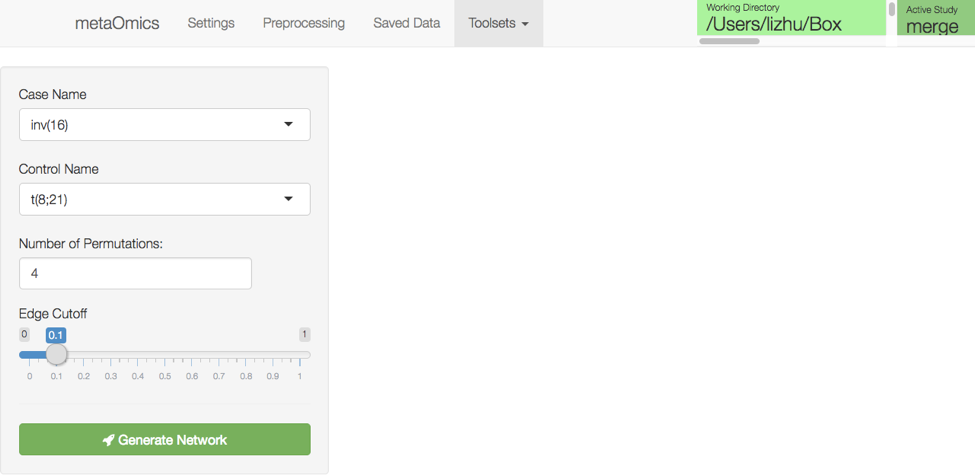
\includegraphics[scale=0.9]{./figure/MetaNetwork/MetaNetworkHome}
\caption{MetaNetwork homepage}
\label{fig:MetaNetworkHome}
\end{center}
\end{figure}

MetaNetwork includes three steps to get differentially co-expressed networks: generate network, search for basic modules, and assemble supermodules. The left screen is the control panel of step 1. The control panel for next step will show up after the previous step is done.

\subsubsection{Procedure}

\begin{steps}
\item \textbf{Generate Network}
The first step of MetaNetwork is to generate co-expression network. 
In this step, the network for permuted data will also be generated. 
Users need to select case and control names, the number of permutations, and edge cut-off which determines the proportion of edges to be kept in the network. 
After clicking \textbf{Generate Network} button, screen will show message indicating the algorithm is running to generate network.


\item \textbf{Search for basic modules}

The next step is to search basic modules.
Advanced options (recommended not to change) include the number of repeats used for each initial seed modules (``Number of repeat"),
the maximim Monte Carlo steps for simulated annealing algorithm (MC Steps),
and the maximum pairwise Jaccard index allowed for basic modules (Jaccard Cutoff), as shown in Figure~\ref{fig:MetaNetworkstep2}.
After clicking \textbf{Search for basic modules} button, screen will show message indicating the algorithm is running to search for basic modules.
This step is computationally demanding depending on gene size.
After this step is done,
the screen will show a table of basic modules highly connected in cases but lose connections in control and vice versa.

\begin{figure}[H]
\begin{center}
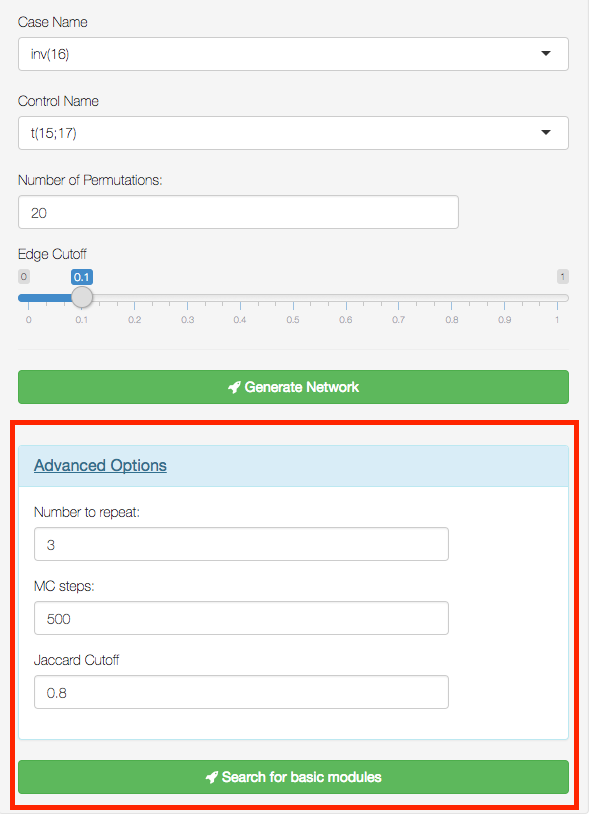
\includegraphics[scale=0.35]{./figure/MetaNetwork/MetaNetworkstep2}
\caption{MetaNetwork control panel for search for basic modules}
\label{fig:MetaNetworkstep2}
\end{center}
\end{figure}

Search for basic modules will take minutes, especially if a large number of genes are used. After this step is done, the screen will show a table of basic modules higher correlated in case and a table of basic modules higher correlated in control as Figure~\ref{fig:MetaNetworkBM}. 

\begin{figure}[H]
\begin{center}
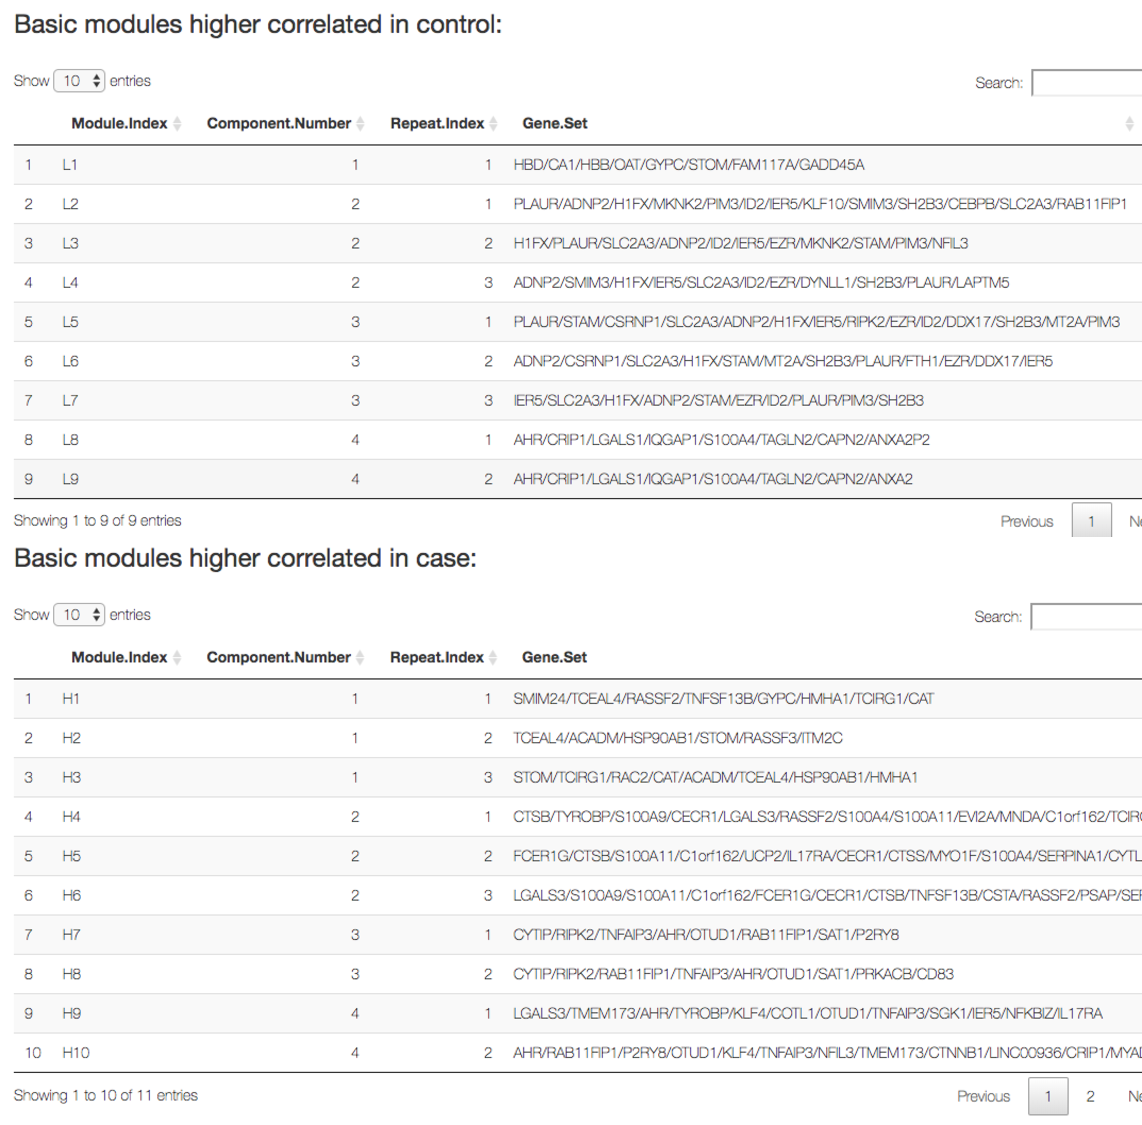
\includegraphics[scale=0.9]{./figure/MetaNetwork/MetaNetworkBM}
\caption{MetaNetwork output from search for basic modules step}
\label{fig:MetaNetworkBM}
\end{center}
\end{figure}

\item \textbf{Assemble supermodules}

After search for basic modules step is done, the control panel will be Figure~\ref{fig:MetaNetworkstep3}. The last step is to assemble supermodules. Users can decide the FDR cut-off to select basic modules for supermodule assembly. 
After clicking \textbf{Assemble supermodules} button, screen will show message indicating the algorithm is running to assemble supermodules.
A table for basic modules, supermodules and their network visualization will be shown on the right panel of screen.
MetaNetwork automatically creates files for top supermodules designed to input to a Cytoscape plug-in ``MetaDCNExplorer"
(\url{http://tsenglab.biostat.pitt.edu/software.htm}) for improved visualization and dynamic exploration.

\begin{figure}[H]
\begin{center}
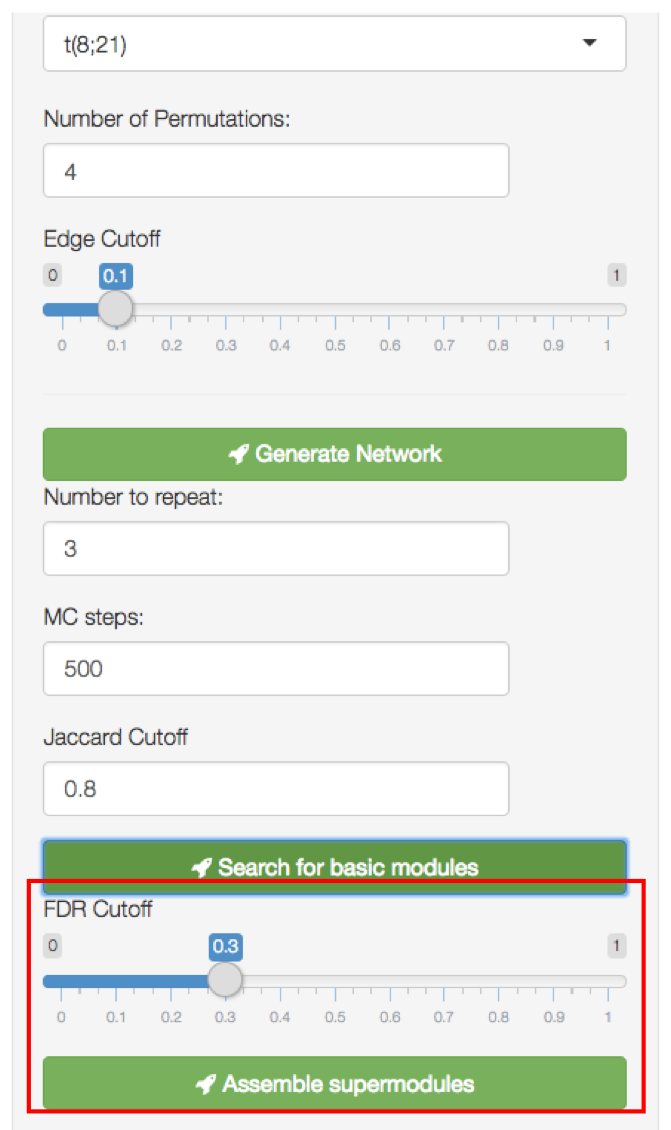
\includegraphics[scale=0.5]{./figure/MetaNetwork/MetaNetworkstep3}
\caption{MetaNetwork control panel for assemble supermodules step}
\label{fig:MetaNetworkstep3}
\end{center}
\end{figure}



\end{steps}

\textbf{Complete List of Options:} 
\begin{enumerate}
\item Generate Network:
\begin{itemize}
\item Case Name: specify case group label.
\item Control Name: specify control group label.
\item Number of Permutations: the number of permutations used for generating network.
\item Edge Cutoff: edge cut-off  determines the proportion of edges to be kept in the network.
\end{itemize}

\item Search for basic modules:
\begin{itemize}
\item Number to repeat:  the number of repeats used for each initial seed modules.
\item MC steps:  the maximum Monte Carlo steps for simulated annealing algorithm.
\item Jaccard cutoff: maximum pairwise Jaccard index allowed for basic modules.
\end{itemize}
\item Assemble supermodules:

\begin{itemize}
\item FDR cutoff:  FDR cut-off to select basic modules for supermodule assembly.
\end{itemize}

\end{enumerate}

\subsubsection{Results}

We used multi-study leukemia gene expression data as example.
After performing merging of the three datasets and filter 80\% genes by mean and 80\% by variance, 206 genes remained.
In this example we only compare two phenotypes: inv(16) and t(8;21).
In general, the MetaNetwork tool is time consuming for large datasets (for both network generation and search for basic modules steps).
We generally suggest users to carefully restrict the number of genes (e.g. less than a thousand) for a test run before implementing large gene set.
By default, all outputs and several interim RData files will be automatically saved to the folder named ``MetaNetwork" under the working directory specified in Section~\ref{sec:setting}.


\textbf{Generate Network}

After the generate network step is done, no output will show up in the screen. Instead, a message box indicating several Rdata files are saved in the MetaNetwork folder, including:

\begin{itemize}
\item AdjacencyMatrices.Rdata is a list of adjacency matrices for case and control subjects in each study. The order is study1 case, study2 case, \dots, studyS case, study1 control, study2 control, \dots, studyS control.
\item CorrelationMatrices.Rdata is a list of correlation matrices for case and control subjects in each study.
\item AdjacencyMatricesPermutationP.Rdata is a list of adjacency matrices for permuted datasets in permutation P.
\end{itemize}

\textbf{Search for basic modules}

After this step is done, the screen will show a table of basic modules higher correlated in case and a table of basic modules higher correlated in control as Figure~\ref{fig:MetaNetworkBM}. Meanwhile, several files will be saved in the MetaNetwork folder:

\begin{itemize}
 \item basic\_modules\_summary\_forward\_weight\_w1.csv is a summary table of basic modules that are higher correlated in case, detected using w1.
 \item basic\_modules\_summary\_backward\_weight\_w1.csv is a summary table of basic modules that are higher correlated in control, detected using w1.
\item threshold\_forward.csv is a table of number of basic modules higher correlated in case, detected under different w1 values and FDR cut-offs.
\item threshold\_backward.csv is a table of number of basic modules higher correlated in control, detected under different w1 values and FDR cut-offs.
 \item permutation\_energy\_forward\_P.Rdata is a list of energies for basic modules that higher correlated in case, detected from permutation P.
  \item permutation\_energy\_backward\_P.Rdata is a list of energies for basic modules that higher correlated in control, detected from permutation P.
\end{itemize}


\textbf{Assemble supermodules}

After supermodule assembly is done, screen will show a table of supermodules (Figure~\ref{fig:MetaNetworksuper}). Users can also select basic modules to plot (Figure~\ref{fig:MetaNetworkBMplot}). Meanwhile several files will be saved in the folder MetaNetwork:
\begin{itemize}
\item module\_assembly\_summary\_weight\_w1.csv is summary table of supermodules using w1 weight.
\item CytoscapeFiles folder contains the input files for Cytoscape to visualize supermodules.
\end{itemize}

\begin{figure}[H]
\begin{center}
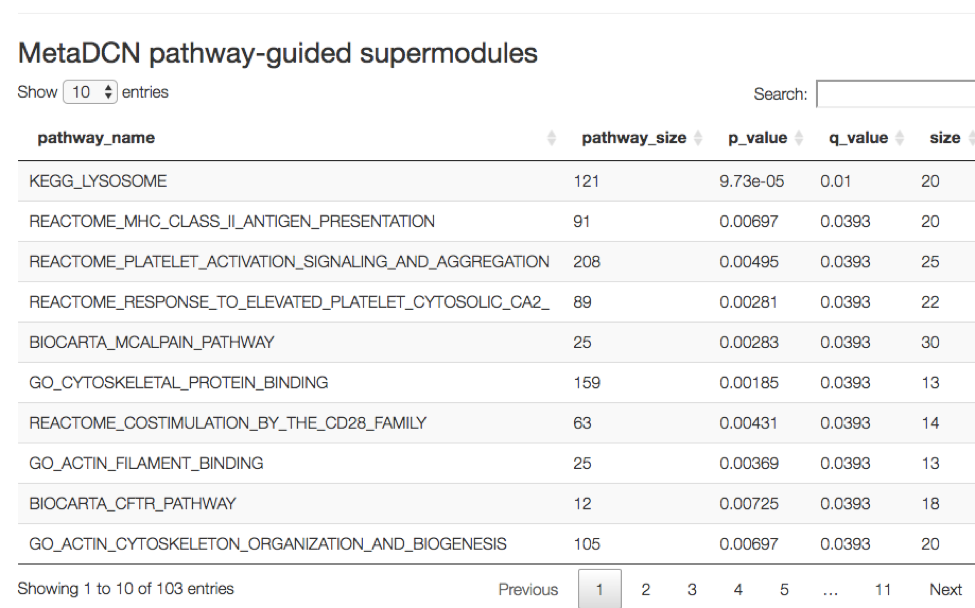
\includegraphics[scale=0.7]{./figure/MetaNetwork/MetaNetworksuper.png}
\caption{MetaNetwork supermodules table}
\label{fig:MetaNetworksuper}
\end{center}
\end{figure}

\begin{figure}[H]
\begin{center}
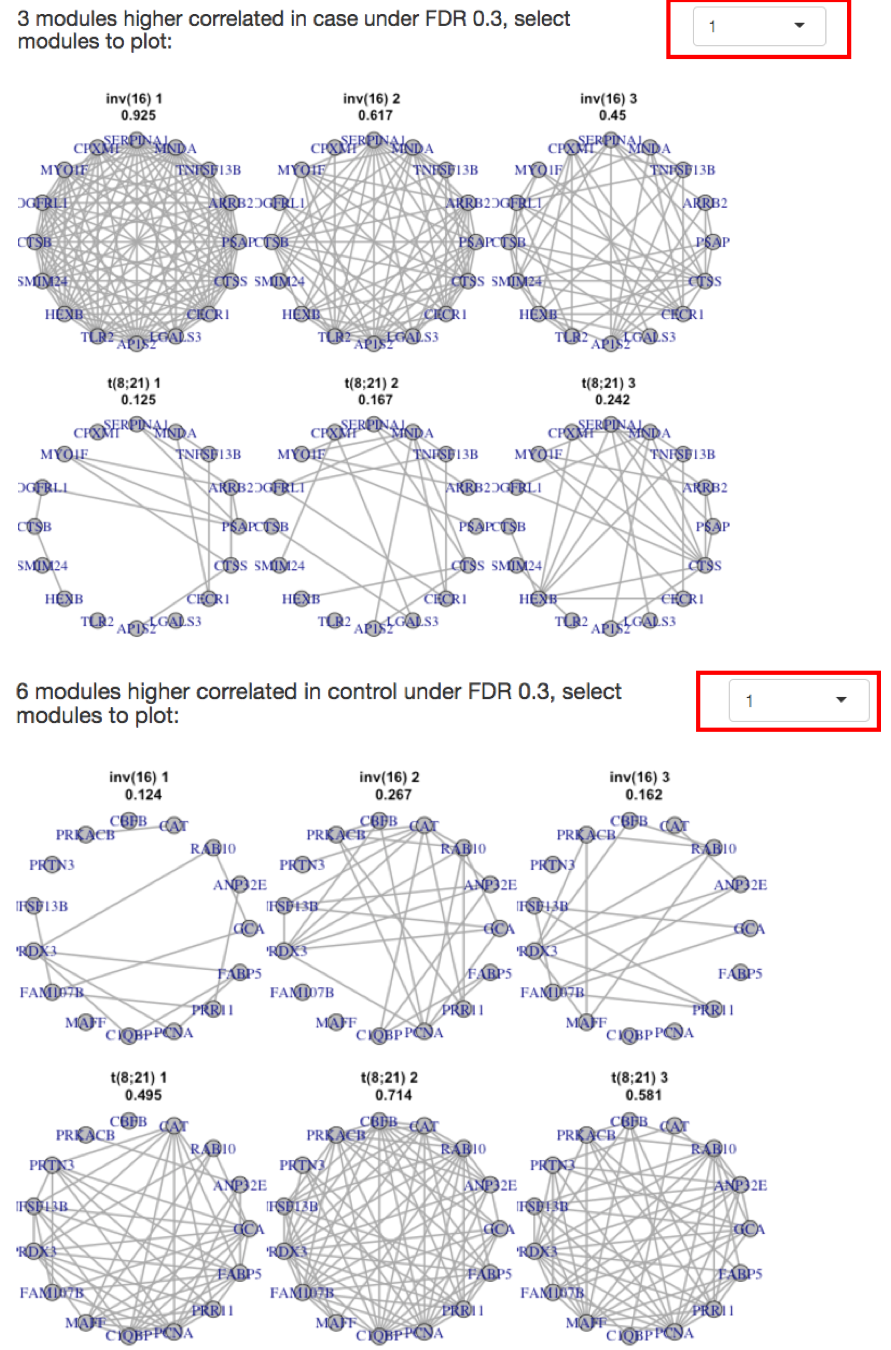
\includegraphics[scale=0.7]{./figure/MetaNetwork/MetaNetworkBMplot.png}
\caption{MetaNetwork select basic modules to plot}
\label{fig:MetaNetworkBMplot}
\end{center}
\end{figure}
